\section{Cache opbygning}
Cachen er opbygget af blokke, af størrelsen $S\cdot E$ elementer. 
En blok ser ud som vist i \cref{fig:cacheblk}
\begin{figure}[h!]
    \centering
    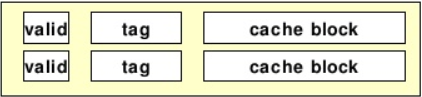
\includegraphics[width=\textwidth]{figures/block.png}
    \caption{Repræsentation af en cache blok}
    \label{fig:cacheblk}
\end{figure}
En sådan blok består af en \textit{Valid} bit, der fortæller om blokken indeholder information, der kan bruges i den givne kontekst.
Der findes også et antal bytes, der gemmer på den ønskede information.
Yderligere indeholder den et markat \textit{tag}, der bruges til at skældne mellem information i cache-linjen, fra hvor det starter i hukommelsen.

For hurtigt at kunne fremsøge information i cachen, opdeles addressen for det ord der ledes efter.
Denne deles i \textit{tag}, \textit{index} og \textit{offset}.
De mindst betydende bits, bruges som offset, de midterste bits bruges til sæt indeks, og de mest betydende bits, bruges til tagget.
For sæt indeks, gælder det at $2^s=S$, altså mængden af sæt i cachen.
Offset vil for et 8-byte ord altid være 3, da offset er 0-indekseret, og derfor ikke må overskride antal gyldige bytes.
Jvf. \cref{tab:bits}.
Dette skyldes at man vil kunne addressere alle bytes i blokken.
De resterende bits, bruges til at danne et tag, for at kunne skældne mellem sæt.

For at kunne tjekke sæt, tag og værdi, kan den givne addresse konverteres til binære tal, hvorved det binære tal kan opdeles i de respektive grupper.
For et 2-byte ord \verb|0xAC| (\verb|1001 1011|), i en cache med 8 sæt, betyder det at strukturen vil se ud som vist i \cref{tab:2byteword}.
\begin{table}[h!]
    \centering
    \begin{tabular}{|c|c|c|c|c|c|c|c|}
        \hline
        7&6&5&4&3&2&1&0\\\hline
        t&t&s&s&s&b&b&b\\\hline
    \end{tabular}
    \caption{Opdeling af 2-byte ord}
    \label{tab:2byteword}
\end{table}
Med denne tabel i tankerne, kan ordet nu opdeles som \verb|10.01 1.011|, hvorved tag, sæt, offset og værdi kan findes.
\textbf{Bemærk} at offset er 0-indekseret.